\documentclass[14pt]{mmcs_article}
\usepackage[russian]{babel}
\usepackage{amsmath, amsthm, amsfonts, amssymb}
\usepackage{tikz}
\usetikzlibrary{shapes, arrows, positioning}
\usepackage{graphicx}
\usepackage{hyperref}
\usepackage{pgfplots}
\pgfplotsset{compat=1.18}
\pgfplotsset{
  every axis/.append style={
    font=\sffamily
  },
  every tick label/.append style={
    font=\sffamily
  },
  every axis label/.append style={
    font=\sffamily
  },
  every axis title/.append style={
    font=\sffamily
  }
}


%\graphicspath{{images/}}%путь к рисункам

\begin{document}

%см. РЕКОМЕНДАЦИИ ПО ОФОРМЛЕНИЮ
%И ПРЕДСТАВЛЕНИЮ КУРСОВЫХ И ВЫПУСКНЫХ %КВАЛИФИКАЦИОННЫХ РАБОТ СТУДЕНТОВ ИНСТИТУТА %МАТЕМАТИКИ, МЕХАНИКИ И КОМПЬЮТЕРНЫХ НАУК


% ----------------------------------
% Внимание!
% Изменяйте только строки, перед которыми стоят знаки комментариев
% ----------------------------------

\thispagestyle{empty}
\begin{singlespacing}
    \begin{center}

        МИНОБРНАУКИ РОССИИ\\ [12pt]
        Федеральное государственное автономное образовательное\\
        учреждение высшего образования\\
        <<Южный федеральный университет>>

        \vspace{\baselineskip}
        Институт математики, механики\\
        и компьютерных наук им.~И.\,И.~Воровича


        \vfill
        % Фамилия Имя Отчество студента
        \textbf{Яценко Артём Алексеевич}

        \vspace{15mm}
        %НАЗВАНИЕ РАБОТЫ должно полностью соответствовать 
        % приказу по ЮФУ (для выпускных квалификационных работ)
        {\bf АВТОМАТИЗАЦИЯ СОПОСТАВЛЕНИЯ \\
            РЕЗЮМЕ И ВАКАНСИЙ}

        \vspace{15mm}
        ВЫПУСКНАЯ КВАЛИФИКАЦИОННАЯ РАБОТА\\
        по направлению подготовки\\
        % Направление обучения 
        02.04.02~-- Фундаментальная информатика и информационные технологии

        \vspace{10mm}
        \textbf{Научный руководитель~--}\\
        % указать данные о руководителе
        % должность, степень, звание Фамилия Имя Отчество
        доц., к.\,ф.-м.\,н. Юрушкин Михаил Викторович

        \vspace{7mm}
        \textbf{Рецензент~--}\\
        % указать данные о рецензенте
        % должность, степень, звание Фамилия Имя Отчество
        доц., к.\,т.\,н. ОТСУТСТВИЕ РЕЦЕНЗЕНТА


        \vspace{15mm}

        \noindent
        % указать Фамилию и инициалы руководителя
        % образовательной программы
        \begin{flushleft}
            Допущено к защите:\\
            руководитель \\
            образовательной программы \underline{\hspace*{60mm}} Демяненко Я.\,М.
        \end{flushleft}




        \vfill
        % год!
        Ростов-на-Дону -- 2025

    \end{center}

    \singlespacing
\end{singlespacing}% для работы магистра

\renewcommand{\contentsname}{Оглавление}

\tableofcontents

%=======================
\newpage
\addcontentsline{toc}{section}{Постановка задачи}

\section*{Постановка задачи}


В постановке задачи коротко (по пунктам) указывается, что необходимо сделать в рамках работы. Раздел <<Постановка задачи>> должен соответствовать заданию на курсовую или выпускную квалификационную работу, подписанному научным руководителем.

%=======================
\newpage
\addcontentsline{toc}{section}{Введение}
\section*{Введение}

Роль информационных систем в процессах рекрутинга и трудоустройства чрезвычайно велика.
В данной работе рассматриваются различные подходы к оптимизации данных процессов с помощью машинного обучения и нейронных сетей.

Одной из наиболее важных задач в процессе рекрутинга является сопоставление кандидатов с вакансиями. Иными словами, среди массива резюме и вакансий необходимо находить такие пары $\langle\text{вакансия},\text{кандидат}\rangle$, которые наиболее соответствуют друг другу (в идеальном случае --- такой кандидат будет принят на предлагаемую должность).
Данная работа рассматривает данную задачу только с точки зрения рекрутера и сфокусирована на поиске кандидатов для определённой вакансии.

У рекрутинговых компаний зачастую присутствует некоторая база данных кандидатов в рамках CRM (candidate relationship management), либо ATS (applicant tracking system) систем.
Стоит отметить, что каждая из компаний использует свои собственные процессы и хранит данные в нестандартизированных форматах.

Таким образом, создание системы для поиска релевантных кандидатов по сути является задачей извлечения и анализа данных из одного или нескольких неструктурированных источников.

Система в таком случае должна возвращать ранжированный список кандидатов, предложенных рекрутеру для конкретной вакансии. Конечно, достичь полной автоматизации процесса поиска соискателей, которые наиболее вероятно будут приняты на определённую работу, достаточно трудно, поэтому рекрутер должен использовать систему как один из инструментов в своей деятельности, а не замену своим профессиональным суждениям.

К тому же, работа рекрутера не ограничивается только лишь приглашением самого подходящего кандидата на работу, так как зачастую приглашенные соискатели могут не пройти одно из собеседований, либо отказаться от предложения. Чтобы максимально эффективно использовать своё время, рекрутер делает так называемый <<screening>>, т.е. выходит на контакт с несколькими кандидатами, и приглашает на собеседование только тех, кто соответствует определённым критериям. При этом количество приглашённых людей рассчитывается <<с запасом>>, на тот случай, что собеседование будет пройдено не всеми из них.

Данные аспекты работы рекрутера вынесены из рассмотрения в данной работе. Рассматривается только задача поиска релевантных соискателей: разрабатываемый подход работает в качестве <<retrieval>> системы, то есть извлекает из базы данных набор резюме для дальнейшего рассмотрения рекрутером и последующей обработки.

Упрощенный процесс поиска кандидатов для вакансии, описанный выше, представлен на рис.~\ref{fig:candidate_search_process}.

\begin{figure}[h]
  \centering
  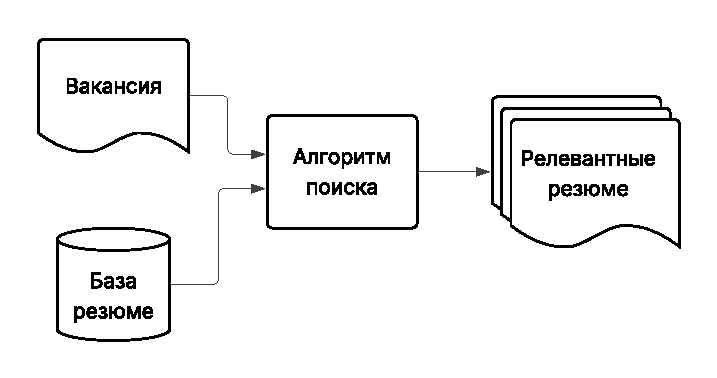
\includegraphics[width=0.8\textwidth]{plots/candidate_search_process.pdf}
  \caption{Процесс поиска кандидатов для вакансии}
  \label{fig:candidate_search_process}
\end{figure}

Очевидно, что улучшение работы алгоритма поиска будет иметь следующие положительные эффекты:

\begin{itemize}
  \item уменьшение количества времени, затрачиваемое рекрутером на поиск кандидатов;
  \item уменьшение времени, затрачиваемого на общение с кандидатами, которые могут не подойти для вакансии по тем или иным причинам
        (освобождение времени для общения с более подходящими кандидатами);
  \item более "точечный" выбор кандидатов, с которыми компания будет выходить на контакт, т.е. меньшее количество <<спама>> кандидатам;
  \item как итог, более эффективная работа компании, увеличение объёма успешно <<закрытых>> вакансий.
\end{itemize}


%=======================
\newpage
\section{Специфика данных}\label{data_specification}

Основные объекты, с которыми ведётся работа в рамках данного исследования --- резюме и вакансии. По своей природе это текстовые данные, не имеющие строгой структуры (очевидно, не существует единого шаблона для резюме).

Тем не менее, некоторые общепринятые понятия, используемые в сфере трудоустройства, можно выделить, и на основе них построить структуру данных. На основе таких общих понятий существует некоторое множество попыток стандартизировать представление резюме и вакансий, зачастую являющиеся XML-схемами (например: \url{https://xmlresume.sourceforge.net/}). Стоит отметить, что ни одна из таких схем не является универсальным стандартом.

В целом, большинство структурированных представлений резюме содержат следующие поля:

\begin{itemize}
  \item Заголовок резюме;
  \item Описание деятельности;
  \item Образование;
  \item Умения (skills);
  \item Опыт работы; несколько записей следующего вида:
        \begin{itemize}
          \item Название должности;
          \item Описание должности;
          \item Дата начала работы;
          \item Дата окончания работы;
          \item Информация о компании;
        \end{itemize}
  \item Сертификаты;
  \item Знание языков;
  \item Персональная и контактная информация;
\end{itemize}

Вакансии намного более сложны в плане структуризации, нежели резюме, так как они зачастую более разнообразны. Однако можно выделить следующие часто встречающиеся поля:

\begin{itemize}
  \item Название вакансии;
  \item Описание вакансии;
  \item Требования (requirements);
  \item Условия (зарплата, график работы, бенефиты);
  \item Контактная информация;
\end{itemize}

Для извлечения указанной информации часто используются так называемые <<парсеры>> --- системы, способные принимать документы во множестве форматов (PDF, DOCX, HTML и т.\,д.) и возвращать их структурированное представление.

Парсинг резюме и вакансий --- отдельная сложная задача, которая не рассматривается в данной работе. Для получения структурированных резюме и вакансий использовался API стороннего сервиса.

\subsection{Фильтрация и ранжирование}\label{filtering_and_ranking}

Исходя из специфики данных, можно разделить задачу поиска релевантных кандидатов на две подзадачи:

\begin{itemize}
  \item Фильтрация резюме;
  \item Ранжирование резюме;
\end{itemize}

Фильтрация заключается в том, чтобы отсеять резюме по каким-либо жестким критериям (пример, если требуется некоторое количество лет опыта с какой-либо технологией, например, Python).

Затем среди отфильтрованных резюме производится ранжирующий поиск. Этот процесс отражён на рис.~\ref{fig:filtering_and_ranking}.

\begin{figure}[h]
  \centering
  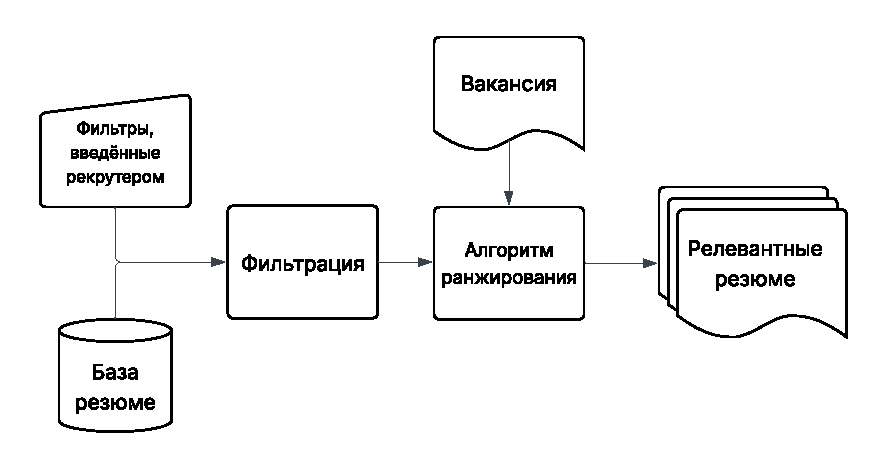
\includegraphics[width=0.8\textwidth]{plots/filtering_and_ranking.pdf}
  \caption{Процесс фильтрации и ранжирования резюме}
  \label{fig:filtering_and_ranking}
\end{figure}

Данный подход имеет свои недостатки.

Одним из таких недостатков является то, что не все кандидаты указывают в своём резюме всю необходимую информацию. Например, если для работы требуются водительские права, то возможность отсеять кандидатов по наличию прав является крайне полезной, однако не все кандидаты явно указывают их наличие (если вы пишете резюме на работу, связанную с вождением, то вы рассчитываете на то, что наличие водительских прав понятно из контекста).

Таким образом, задача фильтрации является сложной задачей, которая требует от системы хорошего понимания содержимого резюме. Иначе, существует риск отсеять кандидата, который является подходящим для вакансии.

Это можно нивелировать, если делать так называемые <<мягкие фильтры>>, которые будут участвовать в ранжировании, но не будут жёстко отсеивать кандидатов. Мягкие фильтры также в какой-то мере отражают то, как рекрутер рассматривает резюме: например, если для работы необходимо пять лет опыта работы в какой-то сфере, то резюме человека, работающего в этой сфере четыре года, будет рассмотрено, и если кандидат обладает достаточной экспертизой, то он будет продвинут в списке кандидатов.

Однако в данной постановке задачи не рассматривается подход <<мягких фильтров>> по следующим причинам:

\begin{itemize}
  \item это усложняет задачу ранжирования, так как необходимо учитывать предпочтения рекрутера (допустим, если требование к годам опыта работы не является жёстким, то актуальным становится вопрос, какую функцию использовать для снижения веса резюме кандидата с опытом, отличным от требуемого на N лет);
  \item <<мягкие фильтры>> являются неочевидными с точки зрения UX, так как пользователи зачастую приходят в замешательство, видя кандидата, который явно не соответствует введённым критериям;
\end{itemize}

Фильтрация нечётким образом могла бы быть <<спрятана>> в ранжирующей модели (например, с помощью преобразования вакансии в набор фильтров с помощью LLM), что позволило бы избежать проблем с UX, однако это является плохим бизнес-решением, так как рекрутеры желают иметь максимально точный контроль над системой.

Таким образом, был выбран подход с жёсткими фильтрами, так как он легко объясним с точки зрения UX (каждый человек ожидает от фильтров именно жёсткого поведения, ведь они повсеместно встречаются в Интернете: например, в интернет-магазинах) и лёгок в реализации.


%=======================
\newpage
\section{Эмбеддинговые модели и векторный поиск}\label{embedding_models}

Так как и вакансия, и резюме являются структурированными текстовыми данными, то для их обработки можно использовать методы NLP (natural language processing).

При этом налагаются следующие ограничения:

\begin{itemize}
  \item каждый запрос должен быть достаточно быстрым и дешёвым; система не может позволить себе оценивать каждого кандидата с помощью LLM;
  \item обработка каждого резюме не должна быть слишком дорогой, т.к. зачастую компании хранят у себя миллионы резюме;
  \item ранжирование должно быть <<умным>>, т.е. учитывать семантику текстов. Алгоритмы, основанные на текстовом совпадении (например, BM-25) являются недостаточно хорошим решением для этой задачи.
\end{itemize}

Исходя из этих ограничений, был выбран подход с использованием эмбеддинговых моделей и векторного поиска.

Эмбеддинговые модели позволяют представить текст в виде вектора чисел фиксированной размерности (обычно от 384 до 1536 измерений). Основная идея такого представления заключается в том, что семантически близкие тексты должны иметь близкие векторные представления.

Например, резюме двух Python-разработчиков с похожим опытом работы должны иметь близкие векторные представления, в то время как резюме Python-разработчика и бухгалтера должны иметь сильно различающиеся векторные представления.

Это свойство позволяет свести задачу поиска похожих текстов к задаче поиска близких векторов в многомерном пространстве. При этом близость векторов может быть измерена с помощью метрик, таких как косинусное расстояние или евклидово расстояние.

Важным преимуществом такого подхода является то, что векторное представление текста может быть вычислено один раз и затем использовано многократно. Это позволяет значительно сократить время и стоимость поиска, так как нет необходимости каждый раз заново анализировать текст.

Кроме того, векторные представления позволяют учитывать семантические связи между словами и фразами. Например, если в вакансии требуется опыт работы с "Python", то резюме кандидата с опытом работы с "Django" также может получить высокий ранг, так как векторные представления этих технологий близки (Django является Python-фреймворком).

\begin{figure}[h]
  \centering
  \begin{tikzpicture}
    \begin{axis}[
        width=0.8\textwidth,
        xlabel={Первая компонента},
        ylabel={Вторая компонента},
        scatter/classes={
            python={mark=*,blue},
            java={mark=*,red},
            accounting={mark=*,green}
          }
      ]
      % Python developers cluster
      \addplot[scatter,only marks,scatter src=explicit symbolic] coordinates {
          (-0.6,0.3) [python]
          (-0.4,0.2) [python]
          (-0.2,0.6) [python]
        };
      % Java developers cluster
      \addplot[scatter,only marks,scatter src=explicit symbolic] coordinates {
          (-1,1) [java]
          (-1.2,0.8) [java]
          (-0.8,1.2) [java]
        };
      % Accountants cluster
      \addplot[scatter,only marks,scatter src=explicit symbolic] coordinates {
          (0,-1) [accounting]
          (0.2,-1.2) [accounting]
          (-0.2,-1.2) [accounting]
        };
      \legend{Python-разработчики,Java-разработчики,Бухгалтеры}
    \end{axis}
  \end{tikzpicture}
  \caption{\centering Визуализация векторных представлений резюме в двумерном пространстве}
  \label{fig:embedding_visualization}
\end{figure}

На рис.~\ref{fig:embedding_visualization} представлена упрощённая визуализация векторных представлений резюме, спроецированных на двумерное пространство. Как видно из рисунка, резюме со схожими навыками и опытом работы располагаются близко друг к другу.

\subsection{Обучение эмбеддинговых моделей}

Эмбеддинговые модели часто требуют дообучения (fine-tuning) на конкретной задаче, так как базовые предобученные веса не всегда достигают оптимального результата. Для того чтобы модель могла генерировать качественные векторные представления для требуемой области, необходимо обучить её на наборе данных из этой области.

Одним из наиболее эффективных подходов к обучению эмбеддинговых моделей является метод Triplet Loss. Этот метод основан на идее обучения на триплетах (тройках), состоящих из следующих элементов:
\begin{itemize}
  \item Anchor (якорь) --- базовый элемент, относительно которого происходит сравнение
  \item Positive (позитивный) --- элемент, семантически близкий к якорю
  \item Negative (негативный) --- элемент, семантически далёкий от якоря
\end{itemize}

Цель обучения заключается в том, чтобы расстояние между векторными представлениями якоря и позитивного примера было меньше, чем расстояние между якорем и негативным примером на некоторую величину (margin). Математически это можно выразить следующим образом:

\begin{equation*}
  \centering
  \allowdisplaybreaks[1]
  \begin{split}
    d(a,p) + margin < d(a,n)
  \end{split}
\end{equation*}

где $d(x,y)$ --- функция расстояния между векторами, $a$ --- якорь, $p$ --- позитивный пример, $n$ --- негативный пример.

Закономерно возникает вопрос составления датасета троек (anchor, positive, negative) для обучения.

\subsubsection{Генерация позитивных примеров}\label{positive_examples_generation}

Так как разметка подобных данных дорога (не каждый человек сможет разметить степень того, насколько кандидат подходит вакансии, необходим опыт в HR-сфере), было принято решение извлекать разметку из самих данных (self-supervised подход), без валидации человеком.

Для генерации позитивных примеров в данной работе использовался подход, основанный на анализе карьерного пути кандидатов. Предполагается, что успешные переходы между позициями в карьере человека указывают на схожесть требуемых навыков и компетенций между этими позициями.

При таком подходе каждая новая позиция в карьере кандидата рассматривается как "вакансия" (anchor), а предыдущий опыт работы --- как позитивный пример (positive). Это позволяет автоматически формировать пары семантически близких резюме на основе реальных карьерных переходов.

Очевидно, что люди могут спонтанно сменить род деятельности (например, стать садовником после долгих лет работы программирования на C++), однако во время экспериментов было установлено, что подобный шум не вносит значительных искажений в результат работы модели. К тому же, когда люди составляют резюме для какой-либо вакансии, они включают только относящийся к ней опыт работы и опускают остальной.

\begin{figure}[h]
  \centering
  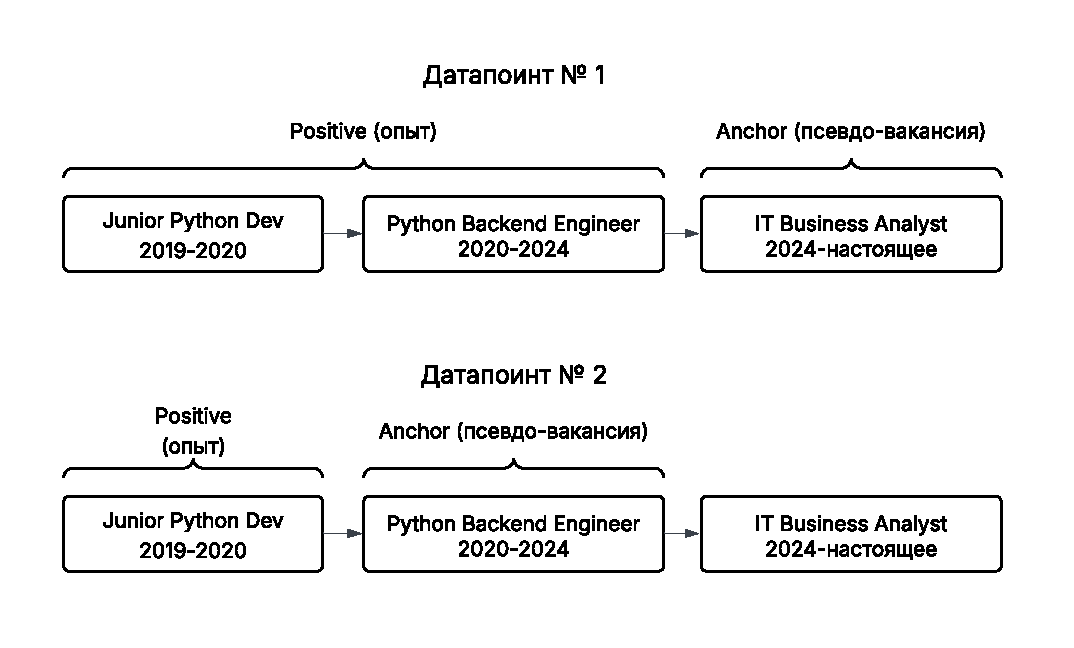
\includegraphics[width=0.8\textwidth]{plots/career_path_example.pdf}
  \caption{Примеры формирования нескольких пар anchor-positive на основе карьерного пути}
  \label{fig:career_path_example}
\end{figure}

Например, как показано на рис.~\ref{fig:career_path_example}, если кандидат успешно продвигался по карьерной лестнице от Junior до IT Business Analyst, то можно считать, что его опыт работы на позиции Junior Python Developer является релевантным для позиции Python Backend Engineer. Также релевантным для позиции IT Business Analyst являлся весь предыдущий опыт, то есть пара $\langle\text{Junior Python Developer},\text{Python Backend Engineer}\rangle$.

Такой подход имеет несколько преимуществ:
\begin{itemize}
  \item Автоматическая генерация большого количества обучающих примеров из реальных данных (а именно N-1 датапоинтов для опыта человека, состоящего из N позиций);
  \item Поиск реальных семантических связей (модель не просто выучит, что Python Developer это хороший кандидат для вакансии Python Developer, но и найдёт связь между Software Engineer и Python Developer).
\end{itemize}

\subsubsection{Аугментация позитивных примеров}

Во время валидации модели были обнаружены некоторые проблемы, требующие решения и переосмысления подхода.
Так как положительный пример и поисковый запрос всегда выбирались из одного резюме, модель переобучалась на стиль написания описаний и названий вакансий. Например, если рекрутер задаёт короткое описание, то будут найдены кандидаты, также не использующие большое количество слов в описаниях опыта.

Таким же образом модель переобучалась и на другие аспекты стиля: lowercase/uppercase, упоминания компаний (если человек множество раз менял должность в рамках одной компании, то это производило достаточно много пар с одинаковыми названиями компаний). Это крайне нежелательно, ведь в таком случае при поиске на работу в какую-либо компанию часть выдачи будет заполнена людьми, уже в ней работающими. Наиболее чётко данный эффект проявлялся тогда, когда кандидат использовал те же специальные символы, что и вакансия (например, звёздочки для обозначения буллит-списков).

Очевидно, что для построения хорошей обучающей выборки необходим препроцессинг, делающий полученную модель инвариантной к стилю написания и анонимизирующий сущности, на которые она может переобучиться.

Этап анонимизации и «стирания» стиля может быть реализован непосредственно перед эмбеддинговой моделью с использованием LLM, что, безусловно, добавит к полученному пайплайну стоимости, так как будет необходим инференс LLM для каждого кандидата.

Было решено не прибегать в препроцессингу с помощью LLM и использовать следующие методы:

\begin{itemize}
  \item Полное удаление специальных символов, <<схлопывание>> множественных пробелов и переносов строк;
  \item Приведение к lowercase;
  \item Использование аугментаций из библиотеки nlpaug.
\end{itemize}

Также рассматривалась возможность использовать NER-подход для нахождения и маскирования PII (personally identifiable information) и названий компаний.

\subsubsection{Генерация негативных примеров}

Одной из основных проблем при использовании Triplet Loss является сложность формирования качественных обучающих триплетов. Если позитивные примеры можно относительно легко получить из реальных данных (например, с помощью указанного выше подхода, либо когда компания приняла кандидата на работу или рекрутер отметил резюме как релевантное), то с негативными примерами ситуация гораздо сложнее. Тот факт, что рекрутер пропустил или не рассмотрел какое-то резюме, не обязательно означает, что данный кандидат не подходит для позиции.

Для эффективного обучения необходимо использовать <<сложные>> негативные примеры --- те, которые достаточно похожи на якорь, но всё же должны быть классифицированы как отличающиеся. В контексте поиска резюме это могут быть, например, резюме специалистов из смежных, но всё же различных областей (например, для резюме Python-разработчика негативным примером может быть резюме системного администратора).

Исходя из подходов к формированию позитивных примеров, описанных в разделе \ref{positive_examples_generation}, поиск качественных негативных примеров становится ещё более сложной задачей. Так как позитивные примеры уже достаточно широкие (учитывая возможность людей менять род деятельности и переходить на смежные позиции), становится труднее найти примеры, которые можно однозначно считать более негативными по отношению к некоторым позитивным.

В рамках данной работы единственным реализуемым способом генерации негативных примеров оказался случайный выбор (random sampling) внутри батча --- резюме, являющиеся позитивными примерами для других якорей в батче, рассматриваются как негативные для текущего якоря. Этот подход продемонстрирован на рисунке \ref{fig:batch_triplets}.

\begin{figure}[h]
  \centering
  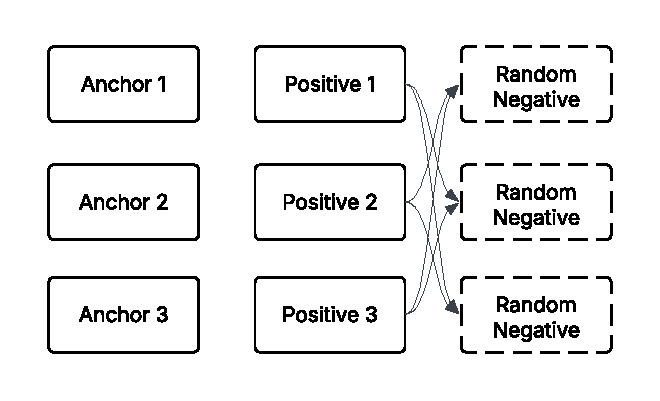
\includegraphics[width=0.8\textwidth]{plots/batch_triplets.pdf}
  \caption{\centering Пример формирования батча из 3-х троек: положительные примеры соседних в батче троек становятся отрицательными для текущего якоря}
  \label{fig:batch_triplets}
\end{figure}

Такой подход к формированию негативных примеров в сочетании с широкими позитивными примерами приводит к появлению ложных отрицательных примеров (false negatives). То есть в некоторых случаях реальный рекрутер мог бы поменять местами позитивный и негативный примеры, так как негативный пример на самом деле более релевантен для данной вакансии. Это является одним из существенных ограничений используемого подхода.

%=======================
\newpage
\section{Ассиметричный поиск}\label{assymetric_search}

В предыдущем разделе был рассмотрен подход к семантическому поиску с использованием эмбеддинговых моделей. Однако, такой подход имеет существенное ограничение --- симметричность метрики косинусного расстояния, используемой для сравнения эмбеддингов. В контексте задачи сопоставления резюме и вакансий это ограничение становится критическим, так как отношения между позициями часто являются асимметричными.

Рассмотрим простой пример: переход от позиции <<Middle Software Engineer>> к <<Senior Software Engineer>> является логичным и желательным с точки зрения карьерного роста. Однако обратный переход --- от <<Senior>> к <<Middle>> --- является нежелательным и даже может быть воспринят как понижение в должности. При использовании традиционного подхода с косинусным расстоянием оба этих перехода будут иметь одинаковую оценку близости, что не соответствует реальной ситуации.

Таким образом, необходимо учитывать не только семантическую близость позиций, но и их относительный <<уровень>> или <<старшинство>>.

Контроль над этим параметром может быть хорошим инструментом для рекрутера, так как в этом случае он смог бы фокусировать поиск на более или менее опытных кандидатах, в зависимости от специфики компании.

\subsection{Требования к асимметричной метрике}

Описанная выше проблема была решена с помощью введения бинарного отношения на множестве позиций ($>_{s}$), которое связывает два элемента множества позиций, если первый элемент является более опытным или старшим по отношению ко второму. Это отношение должно удовлетворять следующим требованиям:

\begin{itemize}
  \item Транзитивность: \\
        \begin{equation*}
          \centering
          \allowdisplaybreaks[1]
          \begin{split}
            \text{Senior developer} & >_{s} \text{Middle developer} \\
                                    & ~~~\land                      \\
            \text{Middle developer} & >_{s} \text{Junior developer} \\
                                    & \implies                      \\
            \text{Senior developer} & >_{s} \text{Junior developer}
          \end{split}
        \end{equation*}
  \item Не все элементы множества позиций должны быть сравнимы друг с другом. Например, трудно определить, является ли <<Middle developer>> более опытным, чем <<Business Analyst>>.
  \item Возможность быстрой проверки того, связывает ли отношение два элемента. Кросс-энкодинг, то есть запуск нейронной сети для каждой пары $\langle p_{job}, p_{candidate} \rangle$ для выявления связи между ними, является достаточно дорогостоящим, поэтому необходимо использовать метод, выполняющий основную массу вычислений на этапе загрузки данных в базу, а не при каждом запросе. Такой метод, например, и используется в описанной выше эмбеддинговой модели (эмбеддинг строится при добавлении данных, а простая операция расчёта косинусного расстояния выполняется во время запроса).
\end{itemize}

Было замечено, что такое отношение может быть реализовано в качестве фильтра в рамках процесса, описанного в разделе \ref{filtering_and_ranking}, то есть кандидаты могут быть отфильтрованы с помощью отношения $>_{s}$, ранжирование может осуществляться эмбеддинговой моделью.

Таким образом, для решения проблемы ассиметричности разработан подход, состоящий из двух компонентов:

\begin{itemize}
  \item Базовая модель семантического поиска, которая находит кандидатов с опытом, схожим с требуемым;
  \item Модель оценки <<старшинства>> (seniority), определяющая относительный уровень позиций в данном участке эмбеддингового пространства.
\end{itemize}

При этом отношение $>_{s}$ выражается отношением <<меньше>> на вещественных числах от 0 до 1 (сравнение чисел транзитивно, выполняется быстро, а эмбеддинговое ранжирование позволяет сравнивать между собой только близкие позиции).

Иными словами, наряду с компонентами эмбеддингов добавляется новая компонента, которая позволяет отфильтровать кандидатов, не соответствующих требованиям по опыту.

Данный подход отражён на рис.~\ref{fig:assymetric_search}.

\begin{figure}[h]
  \centering
  \begin{tikzpicture}
    \begin{axis}[
        view={45}{35},
        axis lines=center,
        xlabel={Первая компонента},
        ylabel={Вторая компонента},
        zlabel={Seniority},
        xlabel style={below right},
        ylabel style={below right},
        zlabel style={rotate=90},
        zmin=0,
        xmin=0.5,
        xmax=1.5,
        ymin=0.5,
        ymax=2.0,
        zmax=2.5,
        xtick=\empty,
        ytick=\empty,
        ztick=\empty,
        width=0.8\textwidth,
        height=0.8\textwidth,
      ]
      % Base points (on the "floor")
      \addplot3[only marks,mark=*,mark size=3pt,color=black] coordinates {
          (1,1,0)  % Python Dev
          (0.7,1.5,0)  % Senior Python Dev
          (0.6,0.7,0)  % Backend Dev
        };

      % Arrows representing seniority
      \addplot3[->,thick,color=red] coordinates {
          (1,1,0) (1,1,0.5)  % Python Dev arrow
        };
      \addplot3[->,thick,color=red] coordinates {
          (0.7,1.5,0) (0.7,1.5,2.0)  % Senior Python Dev arrow
        };
      \addplot3[->,thick,color=red] coordinates {
          (0.6,0.7,0) (0.6,0.7,1.0)  % Backend Dev arrow
        };

      % Labels
      \node[anchor=north west] at (axis cs:1,1,0) {Python Dev};
      \node[anchor=north west] at (axis cs:0.7,1.5,0) {Senior Python Dev};
      \node[anchor=north west] at (axis cs:0.6,0.7,0) {Backend Dev};
    \end{axis}
  \end{tikzpicture}
  \caption{\centering Визуализация асимметричного поиска: точки в эмбеддинговом пространстве с учётом уровня seniority}
  \label{fig:assymetric_search}
\end{figure}

\subsection{Данные для модели ассиметричной оценки}

Для обучения модели был собран датасет, также использующий self-supervised подход. Датасет является набором пар позиций, связанных отношением $>_{s}$.

Эти позиции получены следующим образом:

\begin{itemize}
  \item Была подготовлена база дедуплицированных резюме, где каждая позиция в опыте кандидата была нормализована (приведена к нижнему регистру, удалены спецсимволы и лишние пробелы).
  \item Была создана матрица размера $n \times n$, где $n$ --- количество уникальных позиций в базе резюме. Каждый раз, когда позиция $p_1$ встречалась после позиции $p_2$ в опыте кандидата, элемент матрицы $M[p_1, p_2]$ увеличивался на 1.
  \item После этого для каждой неупорядоченной пары $\langle p_1, p_2 \rangle$ был посчитан коэффициент $k_{p_1, p_2} = \frac{M[p_1, p_2]}{M[p_1, p_2] + M[p_2, p_1]}$.
  \item Были выбраны все пары позиций, для которых $k_{p_1, p_2}$ был выше определённого порога, а так же сумма $M[p_1, p_2] + M[p_2, p_1]$ была достаточно большой, чтобы исключить влияние шума.
\end{itemize}

Примеры таких пар указаны в таблице \ref{tab:seniority_pairs}.

\begin{table}[H]
  \centering
  \caption{Примеры пар позиций, связанных отношением $>_{s}$}
  \label{tab:seniority_pairs}
  \begin{tabular}{|l|l|}
    \hline
    \textbf{"Младшая" позиция} & \textbf{"Старшая" позиция}      \\
    \hline
    Property Manager           & Director of Property Management \\
    \hline
    Accounts Payable Clerk     & Staff Accountant                \\
    \hline
    Business analyst           & Business Analyst Product Owner  \\
    \hline
    Software Engineer          & Senior Database Administrator   \\
    \hline
    Technical Project Manager  & Senior IT Project Manager       \\
    \hline
  \end{tabular}
\end{table}

Из данного датасета была извлечена тестовая выборка. Она составлялась таким образом, чтобы в ней были позиции, которые не встречаются ни в каких отношениях в обучающей выборке.

Достигнуто это было следующим образом: было отобрано некоторое количество позиций, а затем все отношения, в которых они встречались, были помещены в тестовую выборку.

Тестирование на таких позициях крайне важно, так как проверяет способность модели обобщать данные, отслеживать переобучение на распределении конкретных известных позиций.

\subsection{Обучение модели ассиметричной оценки}

Задача свелась к обучению модели регрессии, которая получает на вход одну позицию кандидата и возвращает численную оценку, отражающую уровень опыта.

Сложность обучения такой модели заключается в том, что она должна хранить данные о распределении всех позиций внутри своих весов. Это нужно для того, чтобы видя только одну из двух позиций, она могла произвести для каждой из них оценку, при этом обе оценки должны быть сравнимы друг с другом (больше/меньше), и результат сравнения должен совпадать с отношением $>_{s}$.

В отличие от традиционных задач регрессии, датасет не содержит никаких конкретных чисел, а состоит только из пар позиций и отношений между ними.

Это своего рода уникальная постановка задачи, и может быть обобщена следующим образом:

\begin{itemize}
  \item $P$ --- множество с бинарным отношением $>_{P}$
  \item $I_{P}$ --- множество оценок с обычным отношением порядка $>$, при этом для удобства $I_{P} \subset [0, 1]$
  \item Полученная модель является функцией $f: P \rightarrow I_{P}$, сохраняющей порядок: если $p_{1} >_{P} p_{2}$, то $f(p_{1}) > f(p_{2})$
\end{itemize}

Таким образом, задача сводится к построению монотонного отображения (гомоморфизма упорядоченных множеств) из множества некоторых объектов в множество вещественных чисел с обычным порядком.

При этом данные заданы только лишь парами объектов, удовлетворяющими $>_{P}$.

Оценка качества в таком случае тривиальна: точность (accuracy) на количестве верно предсказанных отношений тестовой выборки.

Однако обучение нетривиально, так как на момент выполнения работы не существовало подходящей лосс-функции для описанной задачи и формата данных.

В ходе экспериментов была разработана собственная лосс-функция, имеющая следующий вид:

\begin{equation}
  \label{eq:custom_loss_function}
  L(p, q) = \begin{cases}
    (p - 0)^2 + (q - 1)^2 & \text{если } \text{margin} + p - q \geq 0 \\
    0                     & \text{иначе}
  \end{cases}
\end{equation}

где:
\begin{itemize}
  \item $p$ --- оценка модели для младшей позиции
  \item $q$ --- оценка модели для старшей позиции
  \item $\text{margin}$ --- константа, определяющая минимально допустимую разницу между оценками
\end{itemize}

Данная лосс-функция пытается <<приблизить>> оценку младшей позиции к нулю, а старшей к единице, если отношение между ними не выполняется с учётом margin.

Реализация процесса обучения с данной лосс-функцией на языке Python с использованием библиотеки HuggingFace представлена в приложении (листинг \ref{app-lst:1}).

У данной лосс-функции, однако, есть один существенный недостаток: Очень медленная сходимость из-за того, что если модель верна, то обучение не происходит вовсе (лосс-функция равна 0). Когда модель становится достаточно хороша и предсказывает >90\% отношений, то огромная часть вычислительных ресурсов, затраченных на инференс модели, не приносит никакой пользы.

Бороться с этим недостатком трудно, так как если штрафовать модель за недостаточную <<уверенность>> в предсказании, то есть продолжать приближать оценки к 0 и 1 даже при правильном предсказании, то это приведёт к тому, что модель не сможет выучить распределение оценок.

Тем не менее, с данной лосс-функцией удалось достичь точности 0.95 на тестовой выборке, то есть модель смогла предсказать более 95\% отношений между позициями.

При этом, обучение модели происходило в течение сотен эпох, что является крайне неэффективным.


\newpage
\section{Ранжирование с учётом опыта}\label{experience_ranking}

Как было показано в предыдущем разделе, наличие отдельного фильтра, позволяющего сравнивать <<старшинство>> позиций, является удобным инструментом для рекрутеров.

Однако, этот инструмент имеет следующие недостатки:

\begin{itemize}
  \item Продемонстрированный способ позволяет сравнивать только пары позиций. При этом резюме являет собой список позиций. Так как модель ассиметричной оценки возвращает численную оценку, то результаты её работы можно агрегировать (например, вычислять среднюю оценку по всем позициям в резюме). Очевидно, что более <<интеллектуальный>> метод оценки всего резюме (а не агрегации отдельных позиций) способен прозводить более точные результаты.
  \item Для реализации предложенного фильтра требуется запустить модель такого же размера, что и эмбеддинговая модель, для каждой позиции из резюме, что довольно затратно.
  \item Обучение модели ассиметричной оценки крайне неэффективно.
\end{itemize}

Обозначенная в разделе \ref{assymetric_search} проблема может быть решена и с помощью другого подхода: если в формате данных для модели сообщить достаточно информации о том, является ли строка резюме или <<вакансией>> (<<вакансия>> взята в кавычки, так как в разделе \ref{positive_examples_generation} было показано, что для обучения псевдо-вакансии извлекаются из резюме), то модель сможет определить, что более <<старшему>> резюме не следует сопоставлять более <<младшие>> вакансии.

Иными словами, если ранее решалась проблема того, что данное равенство нежелательно, но неизбежно вследствие симметричности косинусного расстояния:

\begin{equation}
  \label{eq:assymetric_search_problem}
  \begin{aligned}
    d(\text{junior developer}, & \text{senior developer}) \\
                               & =                        \\
    d(\text{senior developer}, & \text{junior developer})
  \end{aligned}
\end{equation}

где $d$ --- инференс модели для каждого из аргументов и функция расстояния между полученными векторами (косинусное расстояние),

то теперь возможно уйти от данного равенства:

\begin{equation}
  \label{eq:solved_assymetric_search_problem}
  \begin{aligned}
    d(r_{f}(\text{junior developer}), & j_{f}(\text{senior developer})) \\
                                      & \neq                            \\
    d(r_{f}(\text{senior developer}), & j_{f}(\text{junior developer}))
  \end{aligned}
\end{equation}

где:
\begin{itemize}
  \item $r_{f}$ --- функция, преобразующая резюме в формат, понятный модели
  \item $j_{f}$ --- функция, преобразующая вакансию в формат, понятный модели
\end{itemize}

при этом оба формата должны быть достаточно различимы, чтобы модель могла <<классифицировать>>,  с чем имеет дело во время инференса. Приемлемо иметь различные веса для вакансий и резюме, но это несёт дополнительные затраты в виде сложности разработки и не имеет необходимости.






%=======================
\newpage
\section{Описание полученных результатов}\label{dsfs}

В основной части работы должны быть описаны полученные результаты. Здесь возможны:
\begin{itemize}
  \item определения основных понятий, систематизация имеющихся точек зрения по изучаемому вопросу, аргументированная формулировка собственной точки зрения;
  \item теоретические и экспериментальные результаты, полученные автором;
  \item детальные описания методов и алгоритмов решения задач и фактов, лежащих в их основе;
  \item описания разработанных программ, включая образцы экранных\linebreak форм и фрагменты кода.
\end{itemize}

Помимо изложения результатов работа должна содержать методы их получения (доказательства теорем, методика проведения экспериментов, обоснования корректности алгоритмов, и т.\,п.).

В основном тексте также допустимо указывать результаты работы программ, если они имеют небольшой объём. В противном случае эти результаты (или их часть, не вошедшая в основной текст) могут быть приведены в приложениях.


Переносы в заголовках разделов не допускаются.

Необходимо обращать внимание на написание дефисов, длинных и коротких тире в основном тексте, например:

\emph{Одним из участников Великой Отечественной войны и парада Победы на Красной площади в~1945 году был выдающийся российский учёный, чьё имя с гордостью носит наш Институт, и чью столетнюю годовщину со дня рождения мы будем торжественно отмечать 21 июня~--- Иосиф Израилевич Ворович (1920--2001).}


\subsection{Рекомендуемые объёмы работ}

Рекомендуемые объёмы работ приведены в~табл.\,\ref{stud:table:1}. В~скобках указаны рекомендуемые объемы для работ в~области педагогического образования.

\begin{table}[H]
  \centering

  \caption{Рекомендуемые объёмы работ}\label{stud:table:1}

  \begin{tabular}{|p{85mm}|c|}
    \hline
    \multicolumn{1}{|c|}{\bf Уровень работы} &
    \multicolumn{1}{c|} {\bf Объём (в страницах)}              \\
    \hline
    Курсовая работа                          & 8--10 (15--20)  \\
    \hline
    Выпускная квалификационная работа\newline
    (4 курс бакалавриата)                    & 15--20 (40--50) \\
    \hline
    Выпускная квалификационная работа\newline
    (2 год магистратуры)                     & 40--50 (50--70) \\
    \hline
  \end{tabular}
\end{table}



\subsection{Вставка изображений и таблиц}

Все таблицы, рисунки, схемы, диаграммы и другие объекты, вставляемые в текст, должны быть пронумерованы, подписаны и выровнены по центру, в~тексте должна присутствовать ссылка на них (рис.\,\ref{stud:fig:1}).


\begin{figure}[H]
  \centering
  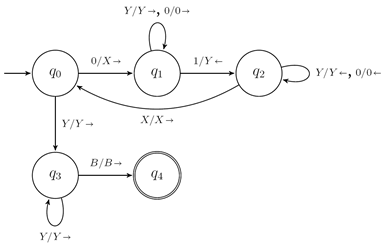
\includegraphics[scale=1.2]{Fig_T.png}
  \caption{Диаграмма переходов машины Тьюринга}\label{stud:fig:1}
\end{figure}


\subsection{Фрагменты исходного кода}

Для иллюстрации излагаемого материала в основной текст можно вставлять фрагменты исходного кода (тексты программ). Они должны быть набраны моноширинным шрифтом (например, \texttt{Courier New}), 12~пунктов, с~одинарным интервалом и выравниванием по левому краю. Если к~фрагментам кода требуется указывать ссылки, их тоже надо снабжать заголовками, как в~случае листингов~\ref{stud-lst:1}--\ref{stud-lst:3}, приведенных ниже.

Если строка кода не помещается на одну строку страницы, её следует разбивать на части в соответствии с принятым стилем форматирования кода, а не автоматически. Размер непрерывных фрагментов исходного кода не должен превышать половины страницы. Фрагменты большего размера следует помещать в приложении к работе.


\subsubsection{Примеры фрагментов кода}

Ниже приведены листинги с заголовками.

\begin{lstlisting}[language=C++, caption={C++, пример кода}, label=stud-lst:1]
#include <iostream>
int main()  // однострочный комментарий
{
  std::cout << "Привет, мир!" << std::endl;
}
\end{lstlisting}


\begin{lstlisting}[language=Python, caption={Python, пример кода}, label=stud-lst:2]
print("Привет, мир!")  # comments
\end{lstlisting}

\begin{lstlisting}[language=TeX, caption=\LaTeX, label=stud-lst:3]
% параметр language в наших листингах только для себя
\bf Привет, мир!
\end{lstlisting}



%=======================
\newpage
\section{Примеры оформления формул}

Внутритекстовая формула
$ \int\limits_a^b f(x)\,dx$ не всегда выглядит красиво даже в \LaTeXe.

Но формулы, вынесенные в отдельную строчку всегда выглядят шикарно
\[
  \lim_{d\to 0} S_n =
  \int\limits_a^b f(x)\,dx.
\]

Для того чтобы {\TeX} автоматически мог ссылаться на нумеруемые формулы нужно указывать команду \verb"\label"
\begin{equation}\label{eq:1}
  \frac{abc}{xyz}.
\end{equation}
Формула (\ref{eq:1}) была оформлена с помощью окружения \textsf{equation}.

%=======================
\newpage
\addcontentsline{toc}{section}{Заключение}
\section*{Заключение}

Заключение должно содержать информацию о проделанной работе и полученных результатах.

При написании текста работы следует иметь в виду, что её цель состоит в том, чтобы продемонстрировать квалификацию автора. Поэтому следует избегать общих и, тем более, тривиальных или нравоучительных высказываний. Мотивация выполняемой работы не должна носить слишком конкретный характер. Во время выступления на защите желательно избегать упоминаний об особенностях стандартных компонентов пользовательского интерфейса программ (<<нажимаем на правую кнопку>>, <<перетаскиваем фрагмент мышью>> и т.\,д.). Не следует комментировать задаваемые после защиты вопросы. Ответы на вопросы должны быть краткими.



%=======================
\newpage

\addcontentsline{toc}{section}{Литература}
\renewcommand{\refname}{\centering \textbf{Литература}}

\begin{thebibliography}{0}
  \bibitem{stud:b0}
  Рекомендации по оформлению
  и представлению курсовых
  и выпускных квалификационных работ
  студентов института математики,
  механики и компьютерных наук.~--
  Ростов н/Д, 2020.

  \bibitem{stud:b1}
  Жуков М.\,Ю., Ширяева Е.\,В.
  \LaTeXe: искусство набора и вёрстки текстов с~формулами.~-- Ростов н/Д : Изд-во ЮФУ, 2009.
\end{thebibliography}


%=======================
\newpage
\section*{Приложение}
\addcontentsline{toc}{section}{Приложение}

\begin{lstlisting}[language=Python, caption={Реализация PairwiseTrainer для обучения модели асимметричной оценки}, tabsize=2, label=app-lst:1, basicstyle=\small\sffamily]
import torch
from transformers import Trainer

MARGIN = 0.01

class PairwiseTrainer(Trainer):
  def get_logits(self, model, inputs):
    input_junior = {
      'input_ids': (
        inputs['input_ids'][:, 0, :].squeeze(dim=1)
      ),
      'attention_mask': (
        inputs['attention_mask'][:, 0, :].squeeze(dim=1)
      ),
    }

    input_senior = {
      'input_ids': (
        inputs['input_ids'][:, 1, :].squeeze(dim=1)
      ),
      'attention_mask': (
        inputs['attention_mask'][:, 1, :].squeeze(dim=1)
      ),
    }
    
    output_junior = model(**input_junior)
    output_senior = model(**input_senior)

    return output_junior, output_senior
  
  def loss_from_logits(self, model,output_junior,  output_senior):
    diff = MARGIN + output_junior - output_senior
    
    junior_loss = model.distance_loss(
      output_junior, 
      torch.zeros_like(output_junior)
    )
    senior_loss = model.distance_loss(
      output_senior,
      torch.ones_like(output_senior)
    )
    
    seniority_loss = torch.where(
      diff >= 0,
      junior_loss + senior_loss,
      diff * 0
    )

    return torch.mean(seniority_loss)

  def compute_loss(self, model, inputs):
    output_junior, output_senior = self.get_logits(
      model, inputs
    )
    return self.loss_from_logits(
      model, output_junior, output_senior
    )
  
  def prediction_step(self, 
    model, 
    inputs, 
    prediction_loss_only, 
    ignore_keys=None
  ):
    with torch.no_grad():
      output_junior, output_senior = self.get_logits(
        model, inputs
        )
      loss = self.loss_from_logits(
        model, output_junior, output_senior
      )
      logits = torch.stack(
        (output_junior, output_senior), 
        dim=1
      ).detach()

      return (loss, logits, torch.ones_like(logits))
\end{lstlisting}


\end{document}
% ----------------------------------------------------------------


\lstset{ %
  language=C++,                 % выбор языка для подсветки (здесь это С++)
  basicstyle=\small\sffamily, % размер и начертание шрифта для подсветки кода
  numbers=left,               % где поставить нумерацию строк (слева\справа)
  numberstyle=\tiny,           % размер шрифта для номеров строк
  stepnumber=1,                   % размер шага между двумя номерами строк
  numbersep=5pt,                % как далеко отстоят номера строк от подсвечиваемого кода
  backgroundcolor=\color{white}, % цвет фона подсветки - используем \usepackage{color}
  showspaces=false,            % показывать или нет пробелы специальными отступами
  showstringspaces=false,      % показывать или нет пробелы в строках
  showtabs=false,             % показывать или нет табуляцию в строках
  frame=single,              % рисовать рамку вокруг кода
  tabsize=2,                 % размер табуляции по умолчанию равен 2 пробелам
  captionpos=t,              % позиция заголовка вверху [t] или внизу [b]
  breaklines=true,           % автоматически переносить строки (да\нет)
  breakatwhitespace=false, % переносить строки только если есть пробел
  escapeinside={\%*}{*)}   % если нужно добавить комментарии в коде
  extendedchars=true,
  commentstyle=\color{mygreen},    % comment style
  stringstyle=\bf,
  commentstyle=\ttfamily\itshape,
  keepspaces=true % пробелы между русскими буквами
  aboveskip=3mm,
  belowskip=3mm

}


\renewcommand\NAT@bibsetnum[1]{\settowidth\labelwidth{\@biblabel{#1}}%
  \setlength{\leftmargin}{\bibindent}\addtolength{\leftmargin}{\dimexpr\labelwidth+\labelsep\relax}%
  \setlength{\itemindent}{-\bibindent+\fivecharsapprox}%
  \setlength{\listparindent}{\itemindent}
  \setlength{\itemsep}{\bibsep}\setlength{\parsep}{\z@}%
  \ifNAT@openbib
    \addtolength{\leftmargin}{\bibindent}%
    \setlength{\itemindent}{-\bibindent}%
    \setlength{\listparindent}{\itemindent}%
    \setlength{\parsep}{0pt}%
  \fi
}
